\documentclass{article}

%----------------------------------------
% Packages
%----------------------------------------
\usepackage[left=1in, right=1in, top=1in, bottom=1in]{geometry}
\usepackage{graphicx}
\usepackage{amsmath,amsbsy,amssymb,amsfonts,amsthm}
\usepackage{nicefrac}
\usepackage{mathtools}
\usepackage{color}
\usepackage{xspace} % Correct macro spacing
\usepackage[numbers]{natbib} % For citations
\usepackage{times}
\usepackage{graphicx,subfigure}
%\usepackage[small,bf]{caption}
\usepackage{algorithm,algorithmic} 
\usepackage{hyperref}

\usepackage{xcolor}
\usepackage{shadethm}

\usepackage{fancyhdr}
\pagestyle{fancy}
\lhead{This is my name}
\rhead{this is page \thepage}

\usepackage{fancyhdr}
\pagestyle{fancy}
\lhead{IFT 6085 - Theoretical principles for deep learning}
\rhead{Lecture 2: January 10, 2019}


\newshadetheorem{thm}{Theorem}
\newshadetheorem{defn}[thm]{Definition}
\newshadetheorem{assm}[thm]{Assumption}
\newshadetheorem{prop}[thm]{Property}
\newshadetheorem{eg}[thm]{Example}
\newshadetheorem{lem}[thm]{Lemma}
\newshadetheorem{cor}[thm]{Corollary}


\definecolor{shadethmcolor}{HTML}{F0F0F0}
%\definecolor{shadethmcolor}{HTML}{EDEDED}
%\definecolor{shadethmcolor}{HTML}{EDF8FF}
%\definecolor{shaderulecolor}{HTML}{EDF8FF}
%\definecolor{shaderulecolor}{HTML}{45CFFF}
\setlength{\shadeboxrule}{.4pt}


\setlength\parindent{0pt}

% Packages hyperref and algorithmic misbehave sometimes.  We can fix
% this with the following command.
\newcommand{\theHalgorithm}{\arabic{algorithm}}

%----------------------------------------
% Standard macros
%----------------------------------------


%----------------------------------------
% Project-specific macros
%----------------------------------------
\DeclareMathOperator*{\argmax}{arg\,max}
\DeclareMathOperator*{\argmin}{arg\,min}

\renewcommand{\vec}[1]{\ensuremath{\boldsymbol{#1}}}
\newcommand{\vecs}[1]{\ensuremath{\mathbf{\boldsymbol{#1}}}}

\newcommand{\mat}[1]{\ensuremath{\boldsymbol{#1}}}
\newcommand{\mats}[1]{\ensuremath{\mathbf{\boldsymbol{#1}}}}

\newcommand{\btheta}[0]{\ensuremath{\boldsymbol{\theta}}}
\newcommand{\bphi}[0]{\ensuremath{\boldsymbol{\phi}}}

\newcommand{\ltheta}[0]{\ensuremath{\mathcal{L}^{(\boldsymbol{\Theta})}}}
\newcommand{\lphi}[0]{\ensuremath{\mathcal{L}^{(\boldsymbol{\Phi})}}}

\newcommand{\phth}[0]{\ensuremath{(\boldsymbol{\phi}, \boldsymbol{\theta})}}
%----------------------------------------
% Header
%----------------------------------------
\title{IFT 6085 - Lecture 14 \\ 
The Numerics of GANs }
\date{}
%----------------------------------------
% Document
%----------------------------------------
\begin{document} 

%----------------------------------------
% Abstract
%----------------------------------------
\maketitle

\vspace{-0.5in}
\begin{center}
This version of the notes has not yet been thoroughly checked.
Please report any bugs to the scribes or instructor.
\end{center}
\vspace{0.2in}

\textbf{Scribes}\hfill
\textbf{Instructor:}  Ioannis Mitliagkas\\
\textbf{Winter 2019:} Adam Ibrahim, William St-Arnaud, Bhairav Mehta \\
\textbf{Winter 2018:} Joshua Romoff


%----------------------------------------
% Body
%----------------------------------------

\newcommand{\infgc}{\inf_{g \in \mathcal{C}}}
\newcommand{\supgc}{\sup_{g \in \mathcal{C}}}

\newcommand{\Prob}{\mathbb{P}}
\newcommand{\E}{\mathbb{E}}
\newcommand{\reals}{\mathbb{R}}

\section{Summary}

In the previous lecture, we discussed the Wasserstein Generative Adversarial Network (WGAN), which uses the Wasserstein distance instead of the traditional Jenson-Shannon divergence. WGANs help alleviate the zero-gradient problem that arises when we have a mismatch in support between the generative and true distribution.
\\

In this lecture, we will focus on the training dynamics for GANs. Specifically, we will frame the training objective for GANs as a zero-sum game, and focus on one particular method, taken from \cite{MeschederNG17a}, that helps GANs convergence to Nash Equilibria. 


\section{Vector fields in optimization}
Traditionally, in optimization, we look for $\btheta^* \in \argmin_{\btheta}\mathcal{L}^{(\btheta)}(\btheta)$ where the loss function $\mathcal{L}$ is smooth and differentiable. A typical strategy consists in looking for stationary points, i.e. points where the gradient of the loss function vanishes (although these may very well be maxima or saddle points too). In practice, gradient descent is often used to find local minima of $\mathcal{L}^{(\btheta)}$. This leads us to consider the vector field $\vec{v}(\btheta)=\nabla\mathcal{L}^{(\btheta)}(\btheta)$.
\begin{defn}[Vector field]
    A vector field is a function mapping a subset of $\mathbb{R}^n$ to $\mathbb{R}^n$. In particular, a vector field $\vec{v}$ is said to be conservative if $\exists f: \mathbb{R}^n \rightarrow \mathbb{R}$ such that $\vec{v} = \nabla f$.
\end{defn}

Since $\vec{v}$ is conservative, the dynamics are straightforward. Indeed, the update rule $F_\eta(\btheta_t) \triangleq \btheta_{t+1} = \btheta_t - \eta \vec{v}(\vec{\btheta_t})$ means that the vector field at each point will point downhill and, if the function is convex, will trace a path to a minimum of the loss function (where $\vec{v}(\btheta) = 0$). We can see from the definition of $F_\eta$ for $\eta \neq 0$ that points where the gradient of $\mathcal{L}$ vanishes (equivalently, stationary points of $\vec{v}$) correspond to fixed points of $F_\eta$, i.e. $\btheta$ such that $F_\eta(\btheta) = \btheta$. One may retrieve convergence guarantees for gradient descent by looking at the Jacobian of $F_\eta$.

\begin{defn}[Jacobian] A generalization of the derivative for vector-valued functions. For $f: \mathbb{R}^n \rightarrow \mathbb{R}^m$, the Jacobian J is defined as:
\[
    J = 
    \begin{bmatrix} 
        \frac{\partial f_1}{\partial x_1} & \dots & \frac{\partial f_1}{\partial x_n} \\
        \vdots & \ddots & \vdots \\
        \frac{\partial f_m}{\partial x_1} & \dots & \frac{\partial f_m}{\partial x_n} 
    \end{bmatrix}
\]
\end{defn} 

The Jacobian of $F_\eta$ is given by $\nabla F_\eta(\btheta) = \mat{I} - \eta \nabla \vec{v}(\btheta)$. Note that $\nabla \vec{v}$ is the Hessian of $\mathcal{L}$, which implies that the Jacobian is symmetric and has real eigenvalues. In this case, the eigenvalues of the Jacobian are directly related to those of the Hessian of $\mathcal{L}$:
\begin{equation}
    \lambda (\nabla F_\eta (\btheta)) = 1 - \eta \lambda(\nabla \vec{v} (\btheta))
\end{equation}
Prop. \ref{prop:bertsekas} provides a local convergence result, based on the spectral radius of the Jacobian of $F_\eta$.

\begin{prop}[Prop. 4.4.1 Bertsekas \cite{Bertsekas/99}] \label{prop:bertsekas}
If the spectral radius $\rho_{max} \triangleq \rho (\nabla F_\eta (\vec{\omega}^*)) < 1$, then, for $\vec{\omega}_0$ in a neighborhood of $\vec{\omega}^*$, the distance of $\vec{\omega}_t$ to the stationary point $\vec{\omega}^*$ converges at a linear rate of $\mathcal{O}\left(\left(\rho_{max} + \epsilon \right)^t\right)$, $\forall \epsilon > 0$.
\end{prop}
In particular, as the spectral radius and the operator 2-norm coincide for symmetric or hermitian matrices, we have that if $\rho (\nabla F_\eta (\btheta^*)) = \max |\lambda (\nabla F_\eta (\btheta^*))| < 1$, fast local convergence is guaranteed by Prop. \ref{prop:bertsekas}.
\par
To illustrate this, consider a quadratic loss $\mathcal{L}^{(\theta)}(\theta) = \frac{h}{2} \theta^2$. Then the vector field is given by $v(\theta) = h\theta$ and its gradient by $\nabla v(\theta) = h$. Thus the eigenvalues of the Jacobian can be easily computed:
\begin{align}
    \lambda(\nabla F_\eta (\theta)) &= 1-\eta \lambda(\nabla v(\theta)) \nonumber \\
    &= 1 -\eta h
\end{align}
Notably, in the case of quadratics, Prop. \ref{prop:bertsekas} is a global convergence result. 


\section{GANs as games}
Recall the min max formulation of GANs,
\begin{equation}
    \min_G \max_D V(D, G) = \E_{x \sim \Prob_x} [\log D(x)] + \E_{z \sim \Prob_z} [\log (1-D(G(z)))]
\end{equation}
GAN optimization can be interpreted as a game, where each player is trying to minimize their own loss function. In that formalism, the goal of training is to find a Nash equilibrium.
\begin{defn}[Nash Equilibrium]
    Given two players parametrized by $\bphi$ and $\btheta$, and their respective loss functions $\lphi \phth$ and $\ltheta \phth$, we say that $\vec{z^*} = (\bphi^*, \btheta^*)$ is a Nash Equilibrium if we have simultaneously:
    \begin{align}
        \bphi^* &\in \argmin_{\bphi\in \vec{\Phi}} \lphi (\bphi, \btheta^*) \nonumber \\
        \btheta^* &\in \argmin_{\btheta\in \vec{\Theta}} \ltheta (\bphi^*, \btheta)
    \end{align}
    As with extremas in optimization, a Nash equilibrium can be local or global. A local Nash equilibrium is a point $\vec{z}^*$ where the above holds in a neighbourhood of $\vec{z}^*$.
\end{defn}
Intuitively, a Nash equilibrium is a point where neither player can improve their situation unilaterally. \\
\par
As the losses involved often are smooth, differentiable, we look for local Nash equilibria using Gradient Descent, which can either update simultaneously the parameters (i.e. $\btheta_{t+1}, \bphi_{t+1}$ only depend on $\btheta_t, \bphi_t$), or alternate updating w.l.o.g. $\btheta$ then $\bphi$ (in which case we may compute $\btheta_{t+1}$ first and then use it instead of $\btheta_t$ to compute $\bphi_{t+1}$). If we consider the vector field
\begin{align}
    \vec{v}\phth = 
    \begin{bmatrix}
        \nabla_{\bphi} \lphi \phth \\
        \nabla_{\btheta} \ltheta \phth
    \end{bmatrix}
\end{align}
one may express the gradient descent update operator as 
\begin{align}
    F_\eta \phth \triangleq \begin{bmatrix}
        \bphi \\
        \btheta
    \end{bmatrix}
    - \eta \vec{v}\phth
\end{align}
Note that in this case the vector field $\vec{v}$ is no longer conservative in general, as in contrast to optimisation, it is no longer the gradient of a real-valued function. In particular, we may observe rotational dynamics. This is due to the fact that the Jacobian is no longer symmetric in general, and may have complex eigenvalues.

For example, consider 
\begin{align}
    \lphi (\phi, \theta) &= \theta \phi, \nonumber \\
    \ltheta (\phi, \theta) &= -\theta \phi
\end{align}
Then, 
\begin{align}
    \vec{v} (\phi, \theta) = \begin{bmatrix}
        \theta \\
        -\phi
    \end{bmatrix},
    \nabla \vec{v} (\phi, \theta) = \begin{bmatrix}
        0 & 1 \\
        -1 & 0
    \end{bmatrix},
    \nabla F_\eta(\phi, \theta) = \begin{bmatrix}
        1 & -\eta \\
        \eta & 1
    \end{bmatrix}
\end{align}
and since the eigenvalues of $\nabla\vec{v}$ are $-i$, $i$, note that applying $\nabla\vec{v}$ 4 times to its eigenvectors yields back the eigenvectors.

\subsection{Zero-sum games}
We assume that we are in the smooth two-player game setting where player $1$ is trying to maximize $f(\vec{\phi}, \vec{\theta})$, player $2$ is trying to maximize $g(\vec{\phi}, \vec{\theta})$, and $f,g$ are both smooth with respect to $\phth$. We also consider the GAN setting which can be cast as a Zero-sum game.
\\

Below describes a notational difference between \cite{MeschederNG17a} and what we saw in class:

\begin{enumerate}
    \item Within the paper, the functions are denoted as $f, g$, whereas in class, we used $\mathcal{L}^{(\Phi)}, \mathcal{L}^{(\Theta)}$. 
    \item \cite{MeschederNG17a} looks at maximizing the functions $f, g$, whereas we are interested in minimization of $\mathcal{L}^{(\Phi)}, \mathcal{L}^{(\Theta)}$. To make these equivalent, we simply note that $$\mathcal{L}^{(\Phi)}(\vec{\phi}, \vec{\theta}) = -f(\vec{\phi}, \vec{\theta})$$
    $$\mathcal{L}^{(\Theta)}(\vec{\phi}, \vec{\theta}) = -g(\vec{\phi}, \vec{\theta})$$
    \item $\mathcal{L} \neq L$; the former denotes the functions we are optimizing, whereas the latter denotes a function of the vector field in \cite{MeschederNG17a}, as we will see below.
    \item The step size in \cite{MeschederNG17a} is denoted as $h$. 
\end{enumerate}

\begin{defn}[Zero-sum games]
\[
    \mathcal{L}^{(\Theta)}(\vec{\phi},\vec{\theta}) = - \mathcal{L}^{(\Phi)}(\vec{\phi},\vec{\theta})
\]
\end{defn}
In zero-sum games, any gain by one player results in a loss to the other player and vice versa; we want to converge to a Nash Equilibrium. Here, the Jacobian of the vector field is given by
\begin{align}
    \nabla\vec{v}\phth= 
    \begin{bmatrix} 
        \nabla^2_{\vec{\phi}} \mathcal{L}^{(\Phi)}(\vec{\phi}, \vec{\theta}) & \nabla_{\vec{\phi}}\nabla_{\vec{\theta}} \mathcal{L}^{(\Phi)}(\vec{\phi}, \vec{\theta}) \\
        - \nabla_{\vec{\phi}}\nabla_{\vec{\theta}} \mathcal{L}^{(\Phi)}(\vec{\phi}, \vec{\theta})^T & - \nabla^2_{\vec{\theta}} \mathcal{L}^{(\Phi)}(\vec{\phi}, \vec{\theta}) 
    \end{bmatrix}
\end{align} 

\begin{lem}
For $0$-sum games, the following are equivalent:
\begin{itemize}
    \item $\nabla\vec{v}(\vec{\phi},\vec{\theta})$ is positive (semi)-definite
    \item $\nabla^2_{\vec{\phi}} \mathcal{L}^{(\Phi)}(\vec{\phi}, \vec{\theta})$ is positive (semi)-definite and $\nabla^2_{\vec{\theta}} \mathcal{L}^{(\Phi)}(\vec{\phi}, \vec{\theta})$ is negative (semi)-definite
\end{itemize}
\end{lem}
Using this lemma for a stationary point of $\vec{v}$ gives a sufficient condition for the existence of a local N.E. Indeed, this is what the following corollary says:
\begin{cor}
The following holds for all $0$-sum games:
\begin{itemize}
\item $\nabla\vec{v}(\vec{\phi}^*,\vec{\theta}^*)$ is positive semi-definite $\forall$ local N.E $(\vec{\phi^*},\vec{\theta^*})$

\item If $(\vec{\phi^*},\vec{\theta^*})$ is a  stationary point of $\vec{v}$ and $\nabla\vec{v}(\vec{\phi^*},\vec{\theta^*})$ is positive definite, then $(\vec{\phi^*},\vec{\theta^*})$ is a local N.E.
\end{itemize}
\end{cor}
Summarizing the previous results, if we have a stationary point $(\vec{\phi^*},\vec{\theta^*})$ of $\vec{v}$, $\nabla_{\vec{\phi}}^2 \mathcal{L}^{(\Phi)}(\vec{\phi},\vec{\theta})$ is positive definite and $\nabla_{\vec{\theta}}^2 \mathcal{L}^{(\Theta)}(\vec{\phi},\vec{\theta})$ is negative definite,  we have that $(\vec{\phi^*},\vec{\theta^*})$ is a local N.E. Now, in the gradient descent algorithm, we compute iterates $(\vec{\phi_{t+1}},\vec{\theta_{t+1}}) = (\vec{\phi_t},\vec{\theta_t}) - \eta \vec{v}((\vec{\phi_t},\vec{\theta_t}))$. Proposition \ref{prop:bertsekas} from the optimization section gives us a convergence guarantee for the gradient descent algorithm. We understand that the convergence rate is dictated by the largest (absolute) eigenvalue. A fixed point signifies that we are in a local optimum. In order to ensure convergence to the local N.E. $(\vec{\phi^*},\vec{\theta^*})$, we must start in a particular neighbourhood $U$ of $(\vec{\phi^*},\vec{\theta^*})$. In other words, we might not get convergence to a local N.E. unless we have a good initial point $(\vec{\phi_0},\vec{\theta_0})$.\\

Recall the issue where  $\nabla\vec{v}$ is not symmetric and therefore the eigenvalues of $F_\eta$ and $\nabla\vec{v}$ are not necessarily real, they can have an imaginary component. The authors of \cite{MeschederNG17a} uncover a sufficient and necessary condition for the conditions of proposition~\ref{prop:bertsekas} to hold.

\begin{lem}[Lemma 4 of Mescheder et al. 2017 \cite{MeschederNG17a}] Assume that $A \in \mathbb{R}^{d\times d}$. If $\forall \lambda \in \sigma(A)$ (where $\sigma(A)$ denotes the spectrum of $A$) we have $Re(\lambda)<0$ and $h>0$ then:
\[
|\lambda| < 1 \quad \forall \lambda \in \sigma(I+hA)
\]
if and only if
\[
h < \frac{1}{|Re(\lambda)|} \frac{2}{1+(\frac{Im(\lambda)}{Re(\lambda)})^2}
\]
\end{lem}

\begin{figure}[h!]
    \centering
    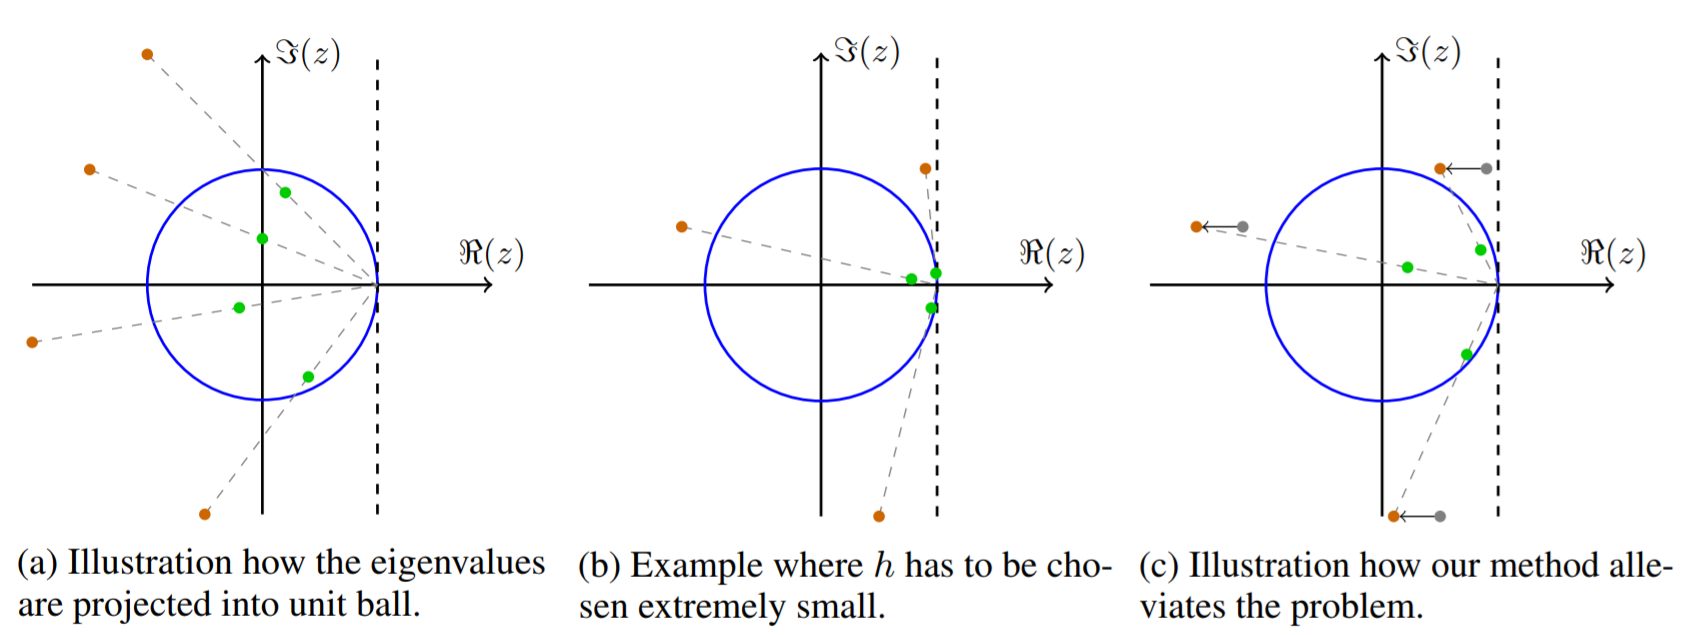
\includegraphics[scale=0.45]{gans.PNG}
    \caption{Illustration of how eigenvalues are shifted into the unit ball for smoother optimization.}
    \label{fig:eval}
\end{figure}

So, in order for the eigenvalues to be within the unit-ball, the learning rate must be made sufficiently small. Figure~\ref{fig:eval} illustrates this effect. If either the real or imaginary component have very large magnitude then a very small learning rate is needed to project the eigenvalues back into the unit ball. 
\\

Since we need to ensure that the eigenvalues stay within the unit ball, we can at each step tune the learning rate or momentum parameter. We can also try to optimize a completely different objective, as shown below. All approaches try to tune the optimization with the hope of making the vector field \textit{more conservative}. Intuitively, we want to control the rotations in the optimization, which will help us converge to local optima faster and more reliably.
\\

\begin{figure}[h!]
    \centering
    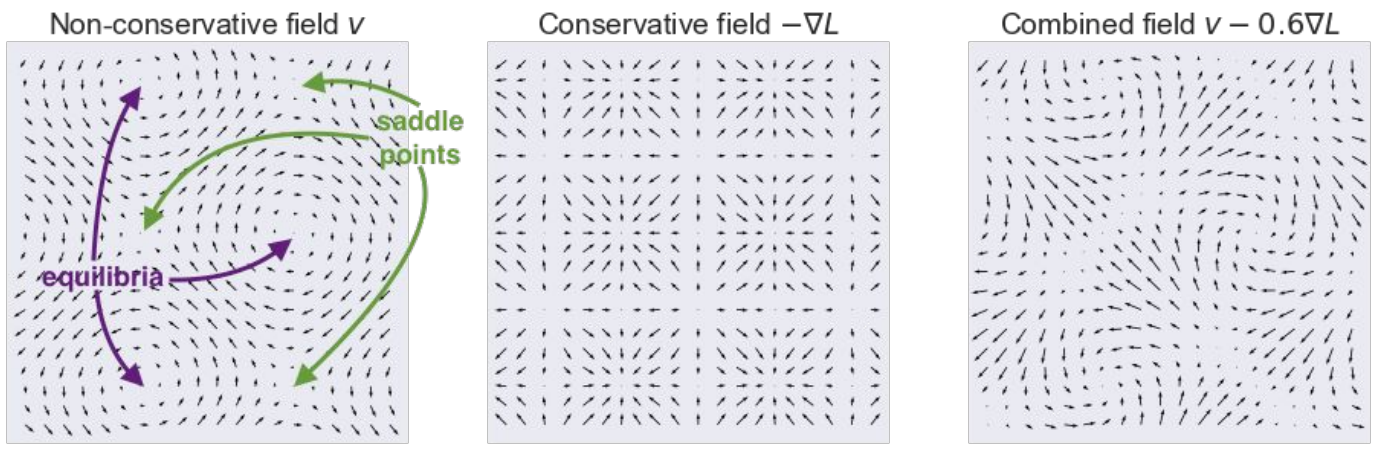
\includegraphics[width=0.8\textwidth]{vectorfieldnog17.png}
    \caption{An illustration of an annotated vector field, conservative field, and the combined field.}
    \label{fig:vfnog}
\end{figure}

The first approach that we can take to tame the rotational dynamics in the vector field is to optimize a completely different objective altogether. As seen in \cite{MeschederNG17a}, we can try to minimize the norm of the gradient. If we have a vector field $\vec{v}$, shown in Panel 1 of Figure \ref{fig:vfnog}, we can optimize the following instead:
\begin{align}
    L(\vec{\phi}, \vec{\theta}) = \frac{1}{2}||\vec{v}(\vec{\phi}, \vec{\theta})||^2
\end{align}

Unfortunately, in practice, this optimization is unstable as the minimization causes saddle points to become attractive, as shown in Panel 2 of Figure \ref{fig:vfnog}.
\\

To solve this issue while still maintaining the benefits of the conservative vector field, the authors propose a gradient penalty, using the above norm of gradient as regularizer controlled by a hyperparameter $\gamma$. In practice, with the right $\gamma$, one can get a combined field that may avoid the false equilibria associated with the conservative field $-\nabla L$ (Panel 3 of Figure~\ref{fig:vfnog}). This combination leads to smoother optimization, as it intuitively scales back the eigenvalues back within the unit ball, while still allowing for larger learning rates.

\section{Negative Momentum}

The previous section showed that for smoother optimization, we need to control the eigenvalues, which can be done by adding a regularizer that shifts the eigenvalues. Effectively, we want to control the rotations in the vector field, which are troublesome as they slow (or prevent) convergence. In this section, we describe the approach taken by \cite{Gidel18NegMom}, which introduces \textit{negative momentum} and describes how it can be used to tame the GAN optimization dynamics.

\subsection{Momentum}
We recall the \textit{heavy ball} method of momentum, originally introduced by \cite{POLYAK19641}:
\begin{align}
\vec{\theta}_{t+1} = \vec{\theta}_t - \eta\vec{v}(\vec{\theta}_t) + \beta(\vec{\theta}_t - \vec{\theta}_{t-1})
\end{align}

where the momentum term is controlled with hyperparameter $\beta$.
\\

In the following, we describe the approach of \cite{Gidel18NegMom}, which provides analysis of \textit{why} large, positive values of momentum are harmful in game optimization, while also providing evidence on how negative momentum (i.e negative values of $\beta$) can be helpful in certain types of zero-sum games.
\\

We begin by rewriting the momentum equation for use with simultaneous, 2-player gradient descent as follows:
$$\vec{x}_{t+1} = \vec{x}_t - \eta\vec{v}(\vec{x}_t) + \beta(\vec{x}_t - \vec{x}_{t-1}), \quad \vec{x}_t = (\vec{\theta}_t, \vec{\phi}_t)$$

Using the above definition, we can also define the fixed point operator, which requires a state-space augmentation.

\begin{align}
    F_{\eta, \beta}(\vec{x}_{t+1}, \vec{x}_t) := 
    \begin{bmatrix}
        \vec{I}_n & \vec{0}_n \\
        \vec{I}_n & \vec{0}_n
    \end{bmatrix}
    \begin{bmatrix}
        \vec{x}_t \\
        \vec{x}_{t-1}
    \end{bmatrix} 
    - \eta 
    \begin{bmatrix}
        \vec{v}(\vec{x}_t) \\
        \vec{0}_n
    \end{bmatrix} 
    + \beta 
    \begin{bmatrix}
        \vec{I}_n & -\vec{I}_n \\
        \vec{0}_n & \vec{0}_n
    \end{bmatrix}
    \begin{bmatrix}
        \vec{x}_t \\
        \vec{x}_{t-1}
    \end{bmatrix} 
\end{align}

\subsection{Negative Momentum in Games}

The paper goes on to show that in a special class of games, called \textit{bilinear games}, a negative momentum parameter can be optimal (and necessary for convergence) for alternated gradient descent (in a bilinear game, simultaneous gradient descent with any choice of momentum parameters may diverge). Figure \ref{fig:bilinearconv} shows an illustration of how negative momentum can lead to convergence with alternated gradient descent, as well as a depiction of how various other methods lead to divergence. 

\begin{figure}[h!]
    \centering
    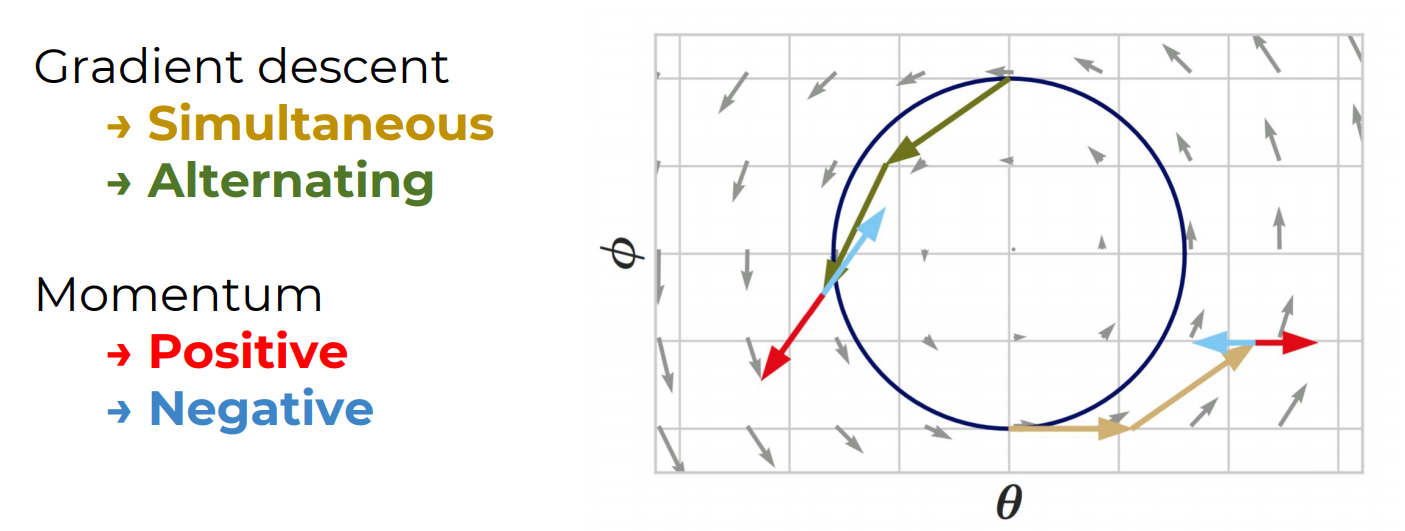
\includegraphics[width=0.8\textwidth]{bilinearconv.png}
    \label{fig:bilinearconv}
    \caption{An illustration of how various choices for gradient descent and momentum parameters lead to different outcomes of optimization.}
\end{figure}


For general games, the paper continues on to show that negative momentum can be helpful as well, and show strong empirical evidence on training "saturating" GANs (i.e. where we get very small or zero gradients) with negative momentum.

%\subsection*{5.2 Noise and Fast Rates}
%
%\begin{prop}[Key Property]
%\[
%	\mathrm{Var}(f) \leq Pf
%\]
%\end{prop}
%Allows faster rates of convergence for $L(g_n^*)- \inf_{g \in \mathcal{C}} L(g)$.
%
%For example, when $\infgc L(g) =0$, then
%\[
%	L(g^*_n) - \infgc L(g) \ll \supgc (L(g) - L_n(g)).
%\]

%----------------------------------------
% \section*{Acknowledgments} 

%----------------------------------------
\bibliographystyle{abbrvnat}
\bibliography{notes}
%----------------------------------------
\end{document}
